\section{Diseño del sistema}

En la figura \ref{fig:chapter_1.overview} vimos un esquema general del sistema, el cual recibe documentos en formato
PDF y genera objetos que contienen la información más importante de los mismos.
En la figura \ref{fig:chapter_1.specific_b} vimos que se va a incluir también el desarollo de dos interfaces, una web
y una de línea de comandos.

En la figura \ref{fig:chapter_4.overview} vemos que el sistema tiene dos componentes principales: el \textit{Reader}
y el \textit{Generator}

\begin{figure}[ht]
    \begin{center}
        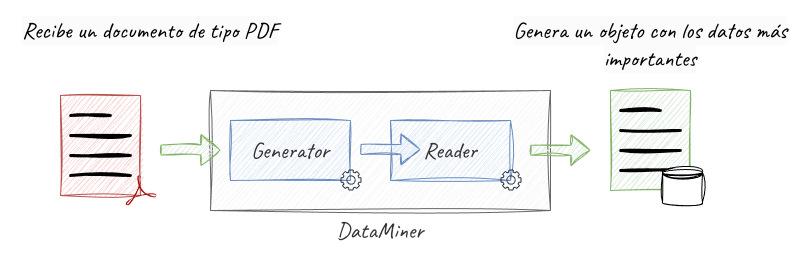
\includegraphics[width=\textwidth]{./chapter/4/images/chapter_4.overview}
        \caption{Esquema de los componentes principales}
        \label{fig:chapter_4.overview}
    \end{center}
\end{figure}

\subsection*{Componente \textit{Generator}}\label{subsec:chapter_4.generator_component}

Este componente sirve como el motor inicial en el proceso, encargado de convertir documentos de cualquier formato a
texto plano.

Se compone de tres conjuntos de elementos y un orquestador al que llamaremos \textit{Engine} responsable de la
coordinación de las operaciones.

Diagrama UML del componente generator.

\subsubsection*{Preprocesadores}
Los preprocesadores preparan el documento original para facilitar su conversión a texto.
En esta implementación no se ha desarrollado ningún preprocesador.

Comunicación del Engine con los preprocesadores definidos.


\subsubsection*{Procesadores}
Actúan como el núcleo del Generator, donde se realiza la conversión efectiva del documento a texto. Funcionan mediante
un sistema competitivo donde varios procesadores evalúan su propia aptitud para manejar el documento en cuestión,
seleccionando el más adecuado para llevar a cabo la tarea.

Este enfoque modular y competitivo asegura que el procesamiento del texto sea no solo eficiente, sino también
extremadamente flexible, adaptándose a las variaciones en la naturaleza de los documentos procesados.


Comunicación del Engine con los procesadores definidos.

En la actual implementación, hemos desarrollado un único procesador especializado en transformar documentos PDF a
texto. Este procesador utiliza la utilidad de línea de comandos `pdftotext` para llevar a cabo la conversión (Glyph \&
Cog, 2023).

\subsubsection*{Postprocesadores}
Estos componentes perfeccionan el texto generado, eliminando errores como caracteres no UTF-8 y espacios en blanco
innecesarios, lo que mejora significativamente la calidad del texto resultante. En esta implementación, se han
desarrollado varios post-procesadores:

\begin{itemize}
    \item
    Word Limit PostProcessor: Se detectó que los elementos de interés, como nombres, documentos de identidad y fechas de
    contratos, típicamente aparecen en las primeras páginas. Este procesador limita el análisis a las primeras N
    palabras del documento.
    \item UTF8 PostProcessor: Implementado tras detectar caracteres no UTF-8 en algunos documentos, este post-procesador
    elimina dichos caracteres.
    \item Character Replace PostProcessor: Desarrollado para eliminar caracteres específicos que complicaba las pruebas.
\end{itemize}

\subsubsection*{Engine}
Este es el orquestador del componente, encargado de hacer las llamadas a los demás elementos registrados en la
aplicación. Coordina el flujo entre los pre-procesadores, procesadores y post-procesadores para asegurar que el
documento sea procesado de manera correcta.

\subsection*{Componente \textit{Reader}}\label{subsec:chapter_4.reader_component}
El componente Reader juega un papel crucial en el proceso de interpretación y procesamiento del texto plano obtenido a
partir de la salida del componente Generator anterior..

Funciona mediante un sistema de procesadores organizados en una única capa, que opera bajo un mecanismo competitivo
similar al del componente Generator. En este sistema, los procesadores compiten entre sí para determinar cuál es el más
adecuado para analizar y extraer la información estructurada necesaria del texto.

Diagrama UML del componente Reader.

\subsubsection*{Procesadores}
Cada uno de estos procesadores es invocado secuencialmente para evaluar su idoneidad en el manejo del documento
específico..

Una vez seleccionado, el procesador elegido procede a ejecutar una serie de tareas que incluyen la identificación y
extracción de entidades clave. En esta implementación, se han desarrollado los siguientes procesadores:

\begin{itemize}
    \item Residential Lease Processor: Evalúa si el documento se trata de un contrato de alquiler de vivienda entre
    particulares. En caso afirmativo, extrae la información más relevante del mismo, como los nombres de los
    arrendadores, los arrendatarios y la fecha del contrato.
    \item Vehicle Sale And Purchase Processor: Evalúa si el documento se trata de un contrato de compraventa de
    vehículos
    entre particulares. En caso afirmativo, extrae la información más relevante del mismo, como los nombres de los
    compradores y vendedores y la fecha de la transacción.
\end{itemize}

\subsubsection*{Engine}
Este es el orquestador del componente, encargado de hacer las llamadas a los demás elementos registrados en la
aplicación, en este caso únicamente los procesadores.


\section{Interfaces de usuario}
Aunque el objetivo principal de este trabajo es desarrollar una tecnología, flexible, extensible y que pueda ser
fácilmente integrada en otros sistemas, se han implementado dos tipos de interfaces sencillas, que permiten demostrar el
correcto funcionamiento de la tecnología.

\subsection*{Interfaz de línea de comandos}
La interfaz de línea de comandos es una herramienta para desarrolladores y administradores del sistema. Permite ejecutar
comandos y scripts de manera directa, facilitando la automatización de tareas y la integración con otros sistemas.


Ejecución de la aplicación a través de la línea de comandos

Esta interfaz recibe como parámetro la ruta de un fichero que se pretende analizar y una vez analizado muestra una
representación en formato tabla de la información extraída del mismo.

\subsection*{Interfaz web}
La interfaz web es el principal punto de interacción para la mayoría de los usuarios. Está diseñada para ser intuitiva,
accesible y eficiente, permitiendo a los usuarios realizar una amplia gama de operaciones a través de un navegador web.

Para este proyecto hemos desarrollado una interfaz con las siguientes características

\begin{itemize}
    \item
    Diseño Responsive: La interfaz web está diseñada para ser accesible desde dispositivos de escritorio y móviles,
    asegurando una experiencia de usuario coherente y optimizada en diferentes tamaños de pantalla.
    \item
    Experiencia de usuario intuitiva: Se ha prestado atención a la usabilidad, con una interfaz limpias y fáciles de
    utilizar y retroalimentación inmediata a las acciones del usuario.
\end{itemize}


Ejecución de la aplicación a través de la interfaz web.

Esta interfaz muestra un área sobre la que se pueden arrastrar y soltar documentos, una vez recibidos, y analizados
muestra una representación en formato json de la información extraída del mismo.


\section{Caché}
La implementación de una caché en aplicaciones web es una técnica comúnmente utilizada para mejorar el rendimiento y la
eficiencia..

En este proyecto, la caché se ha utilizado específicamente para almacenar las peticiones HTTP realizadas, proporcionando
varias ventajas significativas, como el aumento de la velocidad de respuesta y la reducción de costos operativos..

Aunque en un entorno de producción la utilidad de esta caché podría ser limitada, en un entorno de desarrollo resulta
invaluable. Esto se debe a que en desarrollo se trabaja principalmente con un conjunto de datos más pequeño y las
peticiones se repiten con frecuencia.


\section{Registro y gestión de logs}
El registro de logs es una parte crucial del monitoreo y mantenimiento de cualquier aplicación..

En este proyecto, se ha implementado un sistema de logging utilizando Monolog, una biblioteca de registro para PHP.

Además de los logs que almacena symfony por defecto, se han configurado 3 canales adicionales:

\begin{itemize}
    \item Generator: para los logs del componente generator.
    \item Reader: para los logs del componente reader.
    \item Http-Client: para el componente que realiza las peticiones HTTP.
\end{itemize}

Un canal es la forma en la que monolog, agrupa un conjunto de información para poderla filtrar y procesar adecuadamente.

Canal además se registra en dos ficheros diferentes

\begin{itemize}
    \item Log File format, es el formato estándar de ficheros de logs.
    \item Logstash format, es el estándar de la herramienta logstash.
\end{itemize}

\subsection*{Formato de ficheros por defecto}
El formato por defecto es adecuado para entornos de desarrollo o proyectos de pequeña envergadura. Siempre que estos
ficheros no sean demasiado grandes, se pueden trabajar a través de herramientas de línea de comandos como:

\begin{itemize}
    \item grep: Utilizado para buscar patrones específicos dentro de los archivos de logs.
    \item awk: Utilizado para procesar y analizar los logs de manera más compleja.
\end{itemize}

\subsection*{Sistema ELK}
Un sistema compuesto por Elasticsearch, Logstash y Kibana (ELK) es una solución centralizada de gestión de logs, que
permite una monitorización más avanzada de los mismos. Está indicado en entornos de producción, donde la monitorización
de logs sea una tarea importante..


Monitorización de logs a través de un sistema ELK

El sistema ELK se compone de tres componentes:

\begin{itemize}
    \item
    Logstash: Es una herramienta de procesamiento de datos que ingiere, transforma y envía datos a diversos destinos,
    siendo Elasticsearch uno de los más comunes.
    \item
    Elasticsearch: Es un motor de búsqueda y análisis de texto completo basado en Lucene. Permite almacenar, buscar y
    analizar grandes volúmenes de datos en tiempo real.
    \item Kibana: Es una herramienta de visualización de datos que trabaja en conjunto con Elasticsearch. Permite a los
    usuarios crear gráficos y dashboards interactivos para visualizar y analizar los datos de logs almacenados en
    Elasticsearch.
\end{itemize}

\colorbox{color_highlight}{@TODO: @marlene:}
En cuanto a los datos, los generaste manual. No hay forma de generar datos sintéticos? Se podrían generar 100 o 1000
documentos? Sino, hay que justificarlo bien.

\colorbox{color_highlight}{@TODO: @marlene:}
Vale, veo que si usas el LLM de chatgpt. Eso es algo que no me había quedado claro de la memoria. Sin embargo, aún
no
tengo del todo claro qué generas a partir del PDF que recibes. Puedes ejecutar tu herramienta con un contrato? Estás
usando el LLM para extraer los datos del contenido del PDF? Otra pregunta, qué modelo de chatgpt estás usando? Y
puedes
mandar el prompt que usaste?
